%
% 51-kettenzyklen.tex -- Ketten und Zyklen
%
% (c) 2026 Prof Dr Andreas Müller
%
\subsection{Ketten und Zyklen}
Der Integralsatz von Cauchy besagt, dass ein Deformation des Weges
eines Wegintegrals sich nicht auf den Wert des Integrals auswirkt,
solange die Deformation keine Singulartität der Funktion trifft.
%
% fig-paar.tex
%
% (c) 2026 Prof Dr Andreas Müller
%
\begin{figure}
\centering
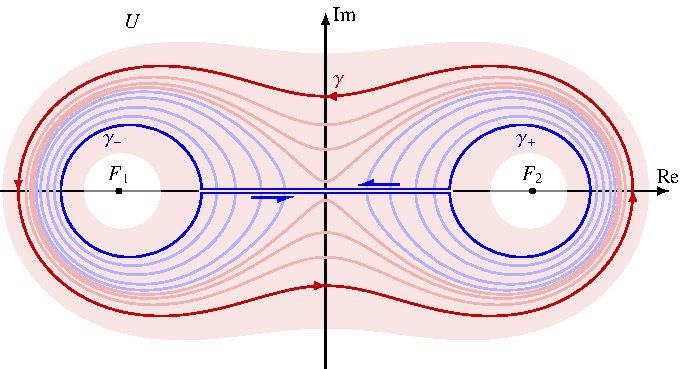
\includegraphics{chapters/030-integration/images/paar.pdf}
\caption{Deformation des Weges $\gamma$ in einen Weg, der die
beiden ``Löcher'' jeweils einmal umlaufen.
Die beiden Wegteile entlang der reellen Achse werden in
entgegengesetzter Richtung durchlaufen, die zugehörigen
Integrale heben sich daher weg.
Der Weg $\gamma$ ist \emph{homolog} zur Summe der Wegen
$\gamma_+$ und $\gamma_-$.
\label{buch:integration:homologie:fig:paar}}
\end{figure}
%
Abbildung~\ref{buch:integration:homologie:fig:paar}
zeigt die Deformation des Pfades $\gamma$, der die beiden ``Löcher''
im Definitionsbereich um die Foki $F_1$ und $F_2$ der Lemniskate
einmal umläuft, in zwei Wege $\gamma_+$ und $\gamma_-$, die $F_1$
und $F_2$ separat umlaufen, verbunden über zwei Wegstücke entlang
der reellen Achse, die in entgegengesetzter Richtung durchlaufen
werden und sich im Integral daher wegheben.
Es folgt, dass
\[
\int_\gamma f(z)\,dz
=
\int_{\gamma_+} f(z)\,dz
+
\int_{\gamma_-} f(z)\,dz.
\]
Wir müssen daher die Idee eines Weges wie $\gamma$ zu einer 
Vereinigung von Wegen wie $\{\gamma_+,\gamma_-\}$ verallgemeinern.

\begin{definition}[Kette]
\label{buch:integration:homologie:def:kette}
Eine \emph{Kette} $C$ in $U$ ist eine formale Summe
\index{Kette}%
\begin{equation}
c
=
c_1\gamma_1 + \dots + c_n\gamma_n
\label{buch:integration:homologie:eqn:def:kette}
\end{equation}
von Wegen $\gamma_k\colon I \to U$ mit $c_k\in\mathbb{Z}$.
Wir bezeichnen mit
\[
C_1
=
C_1
=
\{
c_1\gamma_1+\ldots+c_n\gamma_n
\mid
\gamma_k:I\colon U, c_k\in \mathbb{Z}
\}
\]
die Menge der (eindimensionalen) Ketten.
\end{definition}

Die Definition unterscheidet alle Wege, auch solche, die ineinander
deformierbar sind.
%
% fig-kettenzyklen.tex
%
% (c) 2026 Prof Dr Andreas Müller
%
\begin{figure}
\centering
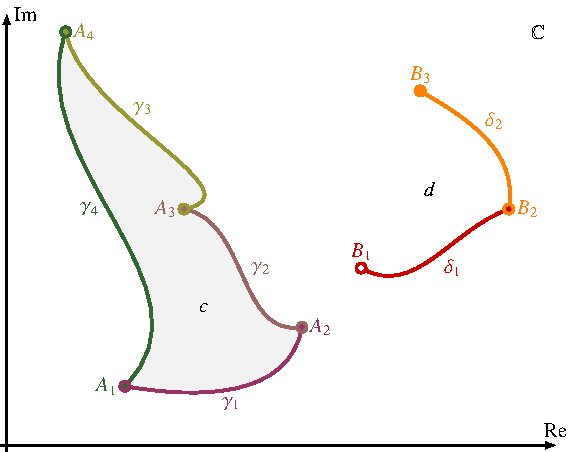
\includegraphics{chapters/030-integration/images/kettenzyklen.pdf}
\caption{Ketten $c=\gamma_1+\gamma_2+\gamma_3+\gamma_4$ und
$d=\delta_1+\delta_2$ sind Linearkombinationen von Wegen.
Der Randoperator extrahiert die Endpunkte mit einem Vorzeichen.
Anfangspunkte sind also offene Kreise, Endpuntke als ausgefüllte
Kreise dargestellt.
Für die Kette $d$ ist $\partial d = B_3-B_1$.
Für die Kette $c$ kommt in $\partial c$ jeder Punkt mit positivem
und negativem Vorzeichen vor, es ist $\partial c=0$.
\label{buch:integration:homologie:fig:kettenzyklen}}
\end{figure}
%
Es wird auch nicht verlangt, dass die Wege geschlossen sind.
Die Wege können geschlossen sein, es kann aber auch sein, dass sich
die Wege zu einem geschlossenen Weg zusammensetzen lassen.

\begin{definition}[Randoperator]
\label{buch:integration:homologie:definition:randoperator}
Die Menge der \emph{$0$-dimensionalen Ketten} ist
\index{Ketten!0-dimensional}%
\[
C_0 
=
C_0(U)
=
\{
c_1P_1+\ldots+c_nP_n
\mid
c_k\in \mathbb{Z}, P_k\in U
\}.
\]
Sie besteht aus formalen Linearkombinationen von Punkten in $U$.
Der \emph{Randoperator} ist eine
\index{Randoperator}%
lineare Abbildung $\partial \colon C_1\to C_0$, die einen
Weg $\gamma$ auf
\[
\gamma \mapsto 1\cdot \gamma(1) - 1\cdot \gamma(0)
\]
abbildet.
\end{definition}

Der Endpunkt eines Weges erhält also das Gewicht $1$, während der
Anfangspunkt das Gewicht $-1$ erhält.
Mehrere Wege können zusammengesetzt werden, wenn der Endpunkt
eines Wegestückes mit den Anfangspunkt des nächsten Stücks
übereinstimmt, wenn also $\gamma_k(1) = \gamma_{k+1}(0)$ gilt.
Der Randoperator bildet $\gamma_k + \gamma_{k+1}$ auf
\[
\partial ( \gamma_k + \gamma_{k+1} )
=
-\gamma_k(0) + \gamma_k(1) -\gamma_{k+1}(0) + \gamma_{k+1}(1)
=
-\gamma_k(0) + \gamma_{k+1}(1)
\]
ab.
Die Zusammensetzbarkeit der Wege ist also genau dann gegeben, 
wenn sich bei Anwendung des Randoperators die Punkte, wo die
Wege zusammengesetzt werden müssen, wegheben.
In Abbildung~\ref{buch:integration:homologie:fig:kettenzyklen}
tritt diese Situation im Zyklus $d$ beim Punkt $B_2$ ein.
Wenn sich alle Punkte wegheben, dann lassen sich die Wegstücke
zu einem geschlossenen Weg zusammensetzen.
In Abbildung~\ref{buch:integration:homologie:fig:kettenzyklen}
tritt dies für den Zyklus $c$ ein.
Wir definieren daher einen Zyklus wie folgt.

\begin{definition}[Zyklus]
\label{buch:integration:homologie:definition:zyklus}
Ein \emph{Zyklus} ist eine Kette in $C_1$, deren Rand verschwindet:
\index{Zyklus}%
\[
Z_1
=
Z_1(U)
=
\{
c\in C_1
\mid
\partial c = 0
\}.
\]
\end{definition}

In Abbildung~\ref{buch:integration:homologie:fig:kettenzyklen} sind
zwei Ketten $c=\gamma_1+\gamma_2+\gamma_3+\gamma_4$ und $d=\delta_1+\delta_2$
dargestellt.
Der Randoperator von $d$ ist
\begin{align*}
\partial d
&=
\partial\delta_1
+
\partial\delta_2
=
B_2-B_1 + B_3-B_2
=
B_3-B_1,
\intertext{es bleiben also die Puntke $B_3$ und $B_1$ mit verschiedenen
Vorzeichen.
Für $c$ ist der Randoperator}
\partial c
&=
\partial \gamma_1
+
\partial \gamma_2
+
\partial \gamma_3
+
\partial \gamma_4
=
A_2-A_1
+
A_3-A_2
+
A_4-A_3
+
A_1-A_4
=
0,
\end{align*}
die Kette $c$ ist also ein Zyklus.
Jeder Teilweg beginnt im Endpunkt eines anderen Weges und endet
im Anfangspunkt eines anderen Weges.
